\chapter{Data analysis}

In this chapter we illustrate the analysis procedure that was followed in this study. A single device under test (DUT) was picked as an example and all the plots in this chapter (unless otherwise stated) refer to the sensor \marginpar{\flushleft add description of all devices analysed} IMEv3-W12, 2x2 array of LGADs.

These main quantities (which will all be properly defined later) were investigated:

% The main part of the analysis followed this path:
\begin{itemize}
    \item Charge
    \item Efficiency
    \item Time resolution
\end{itemize}


\begin{figure}[!hb]
    \centering
    \includegraphics[width=1\linewidth]{Images/plots_of_cuts/Waveform of particle, channel2, with CFD (ns).png}
    \caption{A single pulse with its main features: \textbf{PulseHeight},\textbf{Collected charge}, \textbf{Time of Arrival}}
    \label{fig:waveform_features}
\end{figure} 


\section{Features of the signal}\label{sec:signal_features}

Simplifying the physics \marginpar{\flushleft BIB: pulse of particle passing through} of a particle passing through a thin layer of material: each particle travelling the silicon excites electrons along its path. These electrons drift inside the sensor, guided by an electric field, and create a voltage pulse that can be measured.

An example of such a pulse is shown in Figure \ref{fig:waveform_features}, its most important features were:

\begin{itemize}
    \item PulseHeight\\
The amplitude, or maximum height, of the pulse (in mV).
    \item Charge\\
The total collected charge: integral of the curve, divided by the transimpedance value of the board:
        \begin{equation}
            \text{Charge} = \frac{\int \text{Voltage}(t)dt}{\text{Transimpedance}} \, .
        \end{equation}
    \item Time of Arrival\\
There are several possibilities on how to pick the Time of Arrival (TOA), i.e. the time at which the particle hits the sensor and the pulse is recorded.
The possible choices include: constant threshold discriminator (CTD), constant fraction discriminator (CFD) and zero crossing detector (ZCD); each of these is further explained in Appendix. \marginpar{\flushleft add a short description in the appendix?}
In this study we chose  to use CFD, corresponding to the time when the pulse reaches a certain fraction of the maximum (20\%, 50\% or 70\% in our case).
Furthermore,
\end{itemize}


\section{Positions data}
\marginpar{\flushleft Tracks reconstruction from the MIMOSA planes provide the projected position on the XY plane of each DUT}

\section{Quality cuts}\label{sec:qualtiy_cuts}
To remove the various sources of noise some quality cuts were applied to the data; in this section we explain these choices.

%%% THIS WHOLE PART SHOULD GO LATER
% To get an idea of which events were worthwhile studying we point to two plots (Figures \ref{fig:time_pulseHeight_nocut} and \ref{fig:time_pulseHeight_center}) of the  $\boldsymbol{\Delta t}$ (time of arrival of the DUT - MCP) vs \textbf{pulseHeight}. The left plot shows all of the available tracks (events), the right plot shows only the tracks that pass through the center of the DUT (how this area was selected will be explained in Section \ref{sec:geometry_cut}). The reasoning behind this is that we expect a majority of the noise to come from events whose tracks were outside the boundary of the LGAD, i.e. the event recorded was not matched to a particle hitting the sensor. In this way we managed to identify (and justify) our choices of quality cuts.

% \begin{figure}[!ht]
%     \centering
%     \subfloat[No cuts]{
%         \includegraphics[width=.45\textwidth]{Images/plots_of_cuts/Time_pulseHeight_401S1.png}
%         \label{fig:time_pulseHeight_nocut}}
%     \hfill
%     \centering
%     \subfloat[Center of the sensor]{
%         \includegraphics[width=.5\textwidth]{Images/plots_of_cuts/Time_pulseHeight_401S1 central area.png}
%         \label{fig:time_pulseHeight_center}}
%     \caption{Density plot of events when (left) no cut is applied and (right) when only a central square in the sensor is selected}
% \end{figure}

% After a quick glimpse to plot \ref{fig:time_pulseHeight_nocut} a few peculiarities emerged already, mainly: the constant background noise at low pulseHeight, the main cluster of events with high pulseHeight and the additional "bumps" close to it. By comparing the two plots we could notice that applying a horizontal cut (i.e. a \textit{pulseHeight cut}) could already filter out the majority of the noise.


\subsection{Noise cut}\label{subsec:noise_cut}
The most straightforward trimming consisted in the exclusion of signals which had a pulseHeight less than 3 times greater than the noise\footnote[1]:{For each event, the noise is defined as the standard deviation of the voltage immediately before and after the pulse}
\begin{equation*}
    \text{pulseHeight} > \text{pedestal} + 3\times \text{noise} \, .
\end{equation*}

\subsection{PulseHeight cut}\label{subsec:pulseHeight_cut}

% I think I want to cut out the title
\begin{figure}[!ht]
    \centering
    \includegraphics[width=.5\linewidth]{Images/plots_of_cuts/2D_Sensors_401 S1 pulseHeight cut_pulse.png}
    \caption{PulseHeight cut}
    \label{fig:pulseHeight_cut}
\end{figure}


Firstly, by plotting the distribution of pulseHeight values we applied a cut to the pulses located below the local minimum in the distribution\footnote{A Kernel Density Estimator was used in order to smooth the distribution before identifying the minimum}.
Using this selection of events the X and Y coordinates of the tracks were plotted, giving the result shown in Figure \ref{fig:pulseHeight_cut_highlight}.
The outline is distinctly shown.

Using this information the next cut was implemented, with the goal of selecting only tracks that passed through the surface of the pad, i.e. a \textit{geometry cut}

\subsection{Geometry cut}\label{sec:geometry_cut}

\begin{figure}[!ht]
    \centering
    % \includesvg[width=1\linewidth]{Images/plots_of_cuts/locating_edges_Xtr_batch_401_S1_DUT3}
    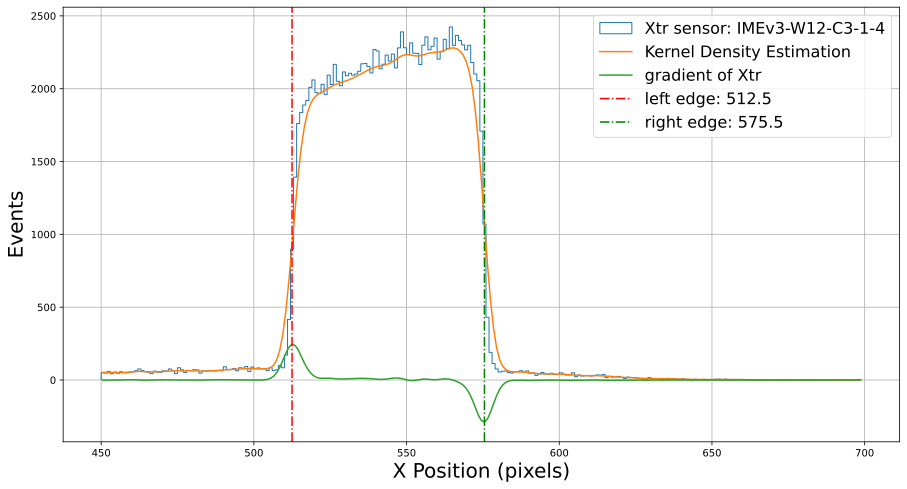
\includegraphics[width=.7\linewidth]{Images/plots_of_cuts/locating_edges_Xtr_batch_401_S1_DUT3.png}
    \caption{How the edges of each sensor were determined}
    \label{fig:edges_of_the_sensor}
\end{figure}

Looking at the projections of hits on the X and Y coordinates, it was possible to determine the outline of the pad. The distribution was smoothed\footnote{Using a Kernel Density Estimator, as done previously for the pulseHeight distribution in Section \ref{subsec:pulseHeight_cut}} and its gradient (derivative) was calculated. This gave rise to two remarkably pronounced peaks shown in Figure \ref{fig:edges_of_the_sensor}, which could be interpreted as the edges of the pads. By applying this procedure to both the X and Y projections we determined the bottom/top and left/right edges, respectively. The final rectangular shape can be seen in Figure \ref{fig:pulseHeight_cut_highlight}, alongside with the density of hits after applying a \textit{pulseHeight cut}. In some cases the sensors were slightly tilted in the XY plane, giving rise to imprecise outlines, this is \marginpar{\flushleft Add later} shown in Appendix although it did not have a significant impact on the rest of the analysis.

% NOTE: the edges defined like this are smaller than the real size of the pad (which is 1.3x1.3 mm$^2$) \cite{Agapopoulou_2022} \marginpar{\flushleft There is an outer guard ring isolating, so maybe the size is correct}

For certain properties that were analyzed (such as efficiency and time resolution) it became clear that the rough selection of the contour of the pad was not always sufficient. Thus, an additional \textit{central area cut} was set up. A region of 0.5x0.5mm$^2$ in the center of the pad was selected (similarly to what had been done in \cite{Agapopoulou_2022}) in order to avoid undesirable effects originating from the region outside the gain layer of the LGAD.

\begin{figure}[!ht]
    \centering
    \subfloat[The heatmap of the reconstructed tracks without any cuts applied. The large rectangular shape is produced by the region of interest (ROI) selected with the FE-I4]{
        \includegraphics[width=.47\linewidth]{Images/plots_of_cuts/2D_Tracks_401 S1 (no cuts)_DUTs_3.png}
        \label{fig:hits_no_cuts}}
    \subfloat[The smaller rectangle corresponding to the area of the pad (highlighted in red with sides lengths) found by applying a \textit{pulseHeight cut}]{
        \includegraphics[width=.45\linewidth]{Images/plots_of_cuts/2D_Tracks_401_S1 highlight geometry cut (using pulseHeight).png}
        \label{fig:pulseHeight_cut_highlight}}
\end{figure}

\subsection{Time cut}\label{sec:time_cut}

Additionally, to further clean the data, a cut on the $\Delta t$ was applied.

Firstly the distribution of $\Delta t$ ($t_{DUT}-t_{MCP}$) without any other cut was fit with a Gaussian plus a uniform background (Figure \ref{fig:time_cut_gauss+bg_fit}):

\begin{figure}[!ht]
    \centering
    \includegraphics[width=.9\linewidth]{Images/plots_of_cuts/time_difference_603_S2_gauss_fit_no_cuts_DUT2.png}
    \caption{Time difference fit with a Gaussian + uniform BackGround}
    \label{fig:time_cut_gauss+bg_fit}
\end{figure}

\begin{equation*}
    f(x,A,\mu,\sigma,BG) = A \cdot e^{-\frac{1}{2}\left(\frac{x-\mu}{\sigma} \right)^2} + BG  \, .
\end{equation*}


$A:$ Amplitude (n° of events);\quad $\mu:$ Mean of the gaussian;\quad $\sigma:$ Standard deviation;\quad $BG:$ Uniform BackGround.

Ultimately, a \textit{time cut} was defined as all the events lying inside an interval of a number \(n\) of standard deviations \(\sigma\):

\begin{equation}
    (\mu-n\sigma;\mu+n\sigma) \, .
\end{equation}

Given that roughly 99.7\% of all values of a normal distribution lie within 3 standard deviations, $n=3$ was deemed an adequate choice.

This cut proved to be especially useful in calculating the total efficiency of each pad and in fitting the charge distribution.

Some peculiarities became apparent, namely the second peak shifted to the right of the main one (meaning delayed compared to the latter) and some discrepancy with the expected Gaussian distribution around the left tail. These were further investigated and will be explained later in Sections \ref{sec:multiple_peaks} and \ref{sec:deviations_from_gaussian}.

\subsubsection{Heavily radiated sensor case}\label{subsec:geometry_cut_w/pulse_cut}

In some cases, typically for heavily radiated sensors, the noise in the pulseHeight distribution was too large (Figure \ref{fig:pulseHeight_cut_failed}) to allow a \textit{pulseHeight cut} as in \ref{subsec:pulseHeight_cut}. This happens due to the pulseHeight decreasing and the noise peaks rising, so the separation bec In these situations it was possible to apply a \textit{time cut} instead and still get a satisfactory contour of the pad. The results betweent the two methods were very similar (Figure \ref{fig:geometry_cut_comparison} in \nameref{chap:appendix}) so this seemed a good alternative.

\begin{figure}[!ht]
    \centering
    \subfloat[PulseHeight distribution]{
        \includegraphics[width=.5\textwidth]{Images/plots_of_cuts/2D_Sensors_603 S2 pulseHeight cut_only_pulse.png}
        \label{fig:pulseHeight_cut_failed}}
    \hfill
    \centering
    \subfloat[Contour of the pad, highlighted in red]{
        \includegraphics[width=.45\textwidth]{Images/plots_of_cuts/2D_Tracks_603_S2 highlight geometry cut (using time).png}
        \label{fig:time_cut_highlight}}
    \caption{Example of a different sensor (\textbf{irradiated}), for which the previous \textit{pulseHeight cut} became impractical (left), but using \textit{time cut} yielded a reasonable outline of the pad (right)}
\end{figure}


\section{Charge distribution}

A central goal of this study was to measure the distribution of the charge collected by the pads and verify their correspondence with the theoretical distribution: a convolution of a Gaussian and a Landau distributions (Appendix \ref{sec:vavilov_vs_landau_distribution})

To achieve this, all of the quality cuts defined in Section \ref{sec:qualtiy_cuts} were applied and a fit with the Gaussian*Landau convolution was carried out (Figure \ref{fig:charge_ROOT_fit}). 

\begin{figure}[!ht]
    \centering
    \includegraphics[width=1\textwidth]{Images/charge_plots/charge_data_all_cuts_401_S1_3_Charge_fit_ROOT_double_plot.png}
    \caption{Fit of the charge distribution}
    \label{fig:charge_ROOT_fit}
\end{figure}

\subsection{Irregularities in the distribution}

\subsubsection{Extra noise}
Despite all the trimming to the data, a noticeable part of the noise centered at $\simeq$ 0 could not be removed. We could not pinpoint the origin of this extra noise but a lot of factors could contribute to it: track reconstruction, other electronic noise etc.
Considering this point, the fit was performed in a smaller interval, avoiding the noise (Figure \ref{fig:charge_ROOT_fit}). The left limit was fixed at $4\si{fC}$, as this is the limit of the signal that the electronic board is able to measure, the right limit was adjusted to include only bins with significant amount of data (and account for the \nameref{subsec:tail_discrepancies})

\subsubsection{Discrepancies in the tail}\label{subsec:tail_discrepancies}
In a few cases the tail of the distribution deviated considerably from the expected function. We were able to successfully explain this discrepancy with the "clipping" effect in some of the pulses, due to the limit set to amplitudes registered by the oscilloscopes.
In Section \ref{sec:pulse_clipping} an example of a clipped pulse and its other aftereffects are shown.

In Figure \ref{fig:charge_vs_pulseHeight_for_clipping} (right) the pulseHeight is plotted against the charge and the clipped events appear very clearly at the rightmost part of the plot. This group of events overlapped with the expected charge distribution and could not be removed without modifying it. For this reason, the only solution was to adjust the range of the fit to try to exclude these events.

\begin{figure}
    \centering
    \includegraphics[width=1\linewidth]{Images/charge_plots/Charge_vs_pulseHeight_density_413_S2_dut3.png}
    \caption{Left: distribution of collected charge with Gaussian*Landau fit. Right: scatter plot PulseHeight vs Charge, revealing the cause of the irregular tail}
    \label{fig:charge_vs_pulseHeight_for_clipping}
\end{figure}

%%% maybe I can put a table to show which cuts I applied to which variables


\section{Efficiency}\label{sec:efficiency}

The efficiency was defined as the total number of tracks with charge larger than a certain \textit{threshold charge} divided by the total number of reconstructed track (\textbf{after} quality cuts had been applied).

\begin{equation*}
    \text{Efficiency} = \frac{\text{Tracks with } q>Q_{threshold}}{\text{Total tracks}}  \, .
\end{equation*}

The threshold charge was chosen to be \(4\si{fC}\), which corresponds to the limit of sensitivity of the ASIC  

Before measuring the overall efficiency of the sensors, we applied a \textit{time cut} (as described in \nameref{sec:time_cut}). Additionally, we elected to restrict the calculation to the smaller \textit{central area} of \(0.5\times0.5\si{mm^2}\) defined earlier in \nameref{sec:geometry_cut}. This area can be seen highlighted in red in Figure \ref{fig:efficiency_2D_plot}, which also shows how the efficiency changes along the surface.

Finally, the total efficiency was computed with different values of \textit{threshold charge} to obtain the plot in Figure \ref{fig:efficiency_depending_threshold}, which shows that (in this example) the value remains constant well after the chosen threshold of \(4\si{fC}\).

\begin{figure}
    \centering
    \includegraphics[width=0.7\linewidth]{Images/efficiency_plots/2D Efficiency_401_S1_with_center_highlight_DUTs_3.png}
    \caption{2D histogram plot of efficiency (per squared bin) and \textit{central area cut} highlighted in red}
    \label{fig:efficiency_2D_plot}
\end{figure}

\begin{figure}
    \centering
    \includegraphics[width=0.5\linewidth]{Images/efficiency_plots/Efficiency depending on threshold charge (with cuts) batch 401 S1.png}
    \caption{Total efficiency when changing the threshold value}
    \label{fig:efficiency_depending_threshold}
\end{figure}


\section{Time Resolution}\label{sec:time_resolution}

The difference of times of arrival between the DUT and the MCP was fitted with a normal distribution. The standard deviation of said distribution corresponded to the time resolution of the DUT and MCP combined. Using simple error propagation, the time resolution of the DUT was computed: 

\begin{equation*}
    \begin{gathered}
    \sigma_{dut+MCP} = \sigma_{dut} \oplus \sigma_{MCP} \\
    \downarrow \\
    \sigma_{dut+MCP}^2 = \sigma_{dut}^2 + \sigma_{MCP}^2 \\
    \sigma_{dut} = \sqrt{\sigma_{dut+MCP}^2-\sigma_{MCP}^2}  \, .
    \end{gathered}
\end{equation*}

For this sensor (Figure \ref{fig:time_resolution_plot}) the final time resolution was \(\sigma_{dut} = 49.38\pm0.81\si{\ps} \)

\begin{figure}
    \centering
    \includegraphics[width=0.7\linewidth]{Images/time_resolution_plots/time_difference_401_S1_zoomed_and_gauss_fit_with_cuts_central_area_DUTs_3.png}
    \caption{Gaussian fit of $\Delta t$ to find the time resolution ($\sigma$), the errorbars are the statistical poissonian error ($y_{err}=\sqrt{N}$)}
    \label{fig:time_resolution_plot}
\end{figure}



\section{Detailed analysis}\label{sec:detailed_analysis}

Some other interesting effects that were investigated further.

\subsection{Multiple peaks}\label{sec:multiple_peaks}

As it was very obvious from Figure \ref{fig:time_cut_gauss+bg_fit}, a second peak appeared in the time distribution.

By picking all the events in a certain time interval and plotting their corresponding reconstructed tracks, we were able to verify that: the main peak simply coincides with the DUT, the second peak arises from events picked up by its neighbouring pad. Figure \ref{fig:time_difference_multiple_peaks_highlight} is evidence of this.
Furthermore, this effect was only observed in DUTs which were part of 2x2 LGAD arrays.

\begin{figure}[!ht]
    \centering
    \includegraphics[width=.7\linewidth]{Images/detailed_analysis/time_difference_401_S1_dut_3_with_both_peaks_simple.png}
    \\ [\smallskipamount]
    \includegraphics[width=.47\linewidth]{Images/detailed_analysis/2D Tracks 401_S1_dut_3_with_first_peak.png}
    \hfill
    \includegraphics[width=.47\linewidth]{Images/detailed_analysis/2D Tracks 401_S1_dut_3_with_second_peak.png}
    \caption{Top: Time distribution with the first and second peak highlighted in yellow and green, respectively.
    Left: Tracks of events inside yellow interval.
    Right: Tracks of events inside green interval. In red is the outline of the DUT as estimated by the \textit{geometry cut} (\ref{sec:geometry_cut}).}
    \label{fig:time_difference_multiple_peaks_highlight}
\end{figure}
\marginpar{\flushleft separate the plots so that the text can fit better}

\subsection{Tail of the time distribution}\label{sec:deviations_from_gaussian}
A secondary effect in the time distribution was the asymmetry between the tails, with the left side notably diverging from a normal distribution. Once again, by singling out only the relevant events, we were able to determine that the ring surrounding the gain layer was responsible for this effect (Figure \ref{fig:time_difference_wide_gaussian}). This further justified our choice of selecting a smaller central area for most of the analysis.

\begin{figure}[!ht]
    \centering
    \includegraphics[width=.55\linewidth]{Images/detailed_analysis/time_difference_401_S1_dut_3_with_wide gaussian_left.png}
    \hfill
    \includegraphics[width=.43\linewidth]{Images/detailed_analysis/2D Tracks 401_S1_dut_3_with_wide_gaussian_base_left.png}
    \caption{Left: selection of of the "wide base" of the distribution.
    Right: Tracks of events inside blue interval}
    \label{fig:time_difference_wide_gaussian}
\end{figure}

\subsection{Pulse clipping}\label{sec:pulse_clipping}

As briefly mentioned before, there was indirect evidence that the pulses recorded by the oscilloscopes had been "cut" at their highest point. To prove this, the waveforms data was investigated and a sample is shown in Figure \ref{fig:clipped_pulse}. The outcomes were:

\begin{itemize}
    \item anomaly in the pulseHeight distribution (Figure \ref{fig:pulseHeight_cut})
    \item irregularities in the charge distribution (Figure \ref{fig:charge_vs_pulseHeight_for_clipping})
\end{itemize}
Fortunately, this effect only impacted a small percentage of the data.

\begin{figure}[!ht]
    \centering
    \includegraphics[width=.9\linewidth]{Images/detailed_analysis/Waveform of clipped pulse (ns).png}
    \caption{Example of a single pulse with the highest section cut out}
    \label{fig:clipped_pulse}
\end{figure}
 
% \subsection{Charge sharing}\label{sec:charge_sharing}


% \subsection{Neighbouring pads}\label{sec:neighbouring_pads}
% \begin{figure}
%     \centering
%     \includegraphics[width=0.5\linewidth]{Images/detailed_analysis/batch 401 duts:3 and 3, edge efficiency studies.png}
%     \caption{Caption}
%     \label{fig:neighbouring_pads}
% \end{figure}


% \subsection{Temperature fluctuations}\label{sec:temperature_fluctuations}


% \subsection{Angle tests}\label{sec:angle_tests}


% \subsection{Radiation damage}\label{sec:radiation_damage}

